%I used overleaf

\documentclass[11pt]{amsbook}

\usepackage{../HBSuerDemir}	

% ------------------------
\begin{document}
% ++++++++++++++++++++++++++++++++++++++
\hPage{b1p2/280}
% ++++++++++++++++++++++++++++++++++++++

$18. \ a) \ 8(y-5) = (x-2)^2, \qquad\qquad\qquad b) \ 8(y+4) = (x-3)^2.$

$20. \ a) \ 16(x-2)^2 \ - \ 9(y-3)^2 = 144, \qquad \ b) \ 36(x+2) \ - \ 64(y-1)^2 = 2324.$
    
\subsection{SECOND DEGREE CURVES (SDC)}
\label{sec:SECOND DEGREE CURVES (SDC)}

\subsubsection{DEFINITIONS AND CLASSIFICATION}

\ 

The equation of a conic C in the general case is obtained by taking the directrix D and focus F arbitrarily in the analytic plane as

  \begin{equation}
  D: f(x,y) = ax + by + c = 0, \ (a^2 + b^2 = 1), \ F(x_0,y_0) \qquad 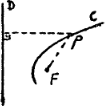
\includegraphics[width=0.15\textwidth]{images/b1p2-280-fig01}
  \end{equation}
  
From

  \begin{equation}
  C = \{P(x,y):d(P,F)/d(P,D) = e\}
  \end{equation}

we have

  \begin{equation}
  \left( (x-x_0)^2 + (y-y_0)^2 )\right/ |ax+by+c|^2 = e^2
  \end{equation}
  
which when expanded and arranged gives the general second degree equation (SDE):

	\begin{equation}
    \label{eq:SDC}
	Ax^2 + Bxy + Cy^2 + Dx + Ey + F = 0, \ (A^2 + B^2 + C^2 \neq 0)
	\end{equation}

as the equation of C where the coefficient A, B, ... , F are functions of constants $a, b, c, x_0, y_0$ and $e$. It follows that the equation of any conic is of second degree, since $A^2 + B^2 + C^2 \neq 0$ But the equation \eqref{eq:SDC} may represent curves other than the conics (ellipse, hyperbola, parabola) as seen from

  \begin{center}
  $(2x - y + l)(x + y - 3) = 0$ %I could not understand which sign is that between x and y (x + y - 3) please check it from book.
  \end{center}

which is of second degree and represents two intersecting lines (0 degenerate conic). % Also not sure is that 0

A curve represented by second degree equation \eqref{eq:SDC} in the variables $x, y$ is called a \textit{second degree curve}. %Is there an "a" exist between "by second"? More than usual space exists there.

The following are, second degree curves: 

\end{document}